\section{Experimental evaluation}

\subsection{Experiment setup}

\subsubsection{Datasets}

The proposed methods were experimentally verified on several datasets. The datasets Cora, CiteSeer and PubMed \cite{yang_revisiting_2016} were used separately both with the fixed public train-test split as in \cite{yang_revisiting_2016} as well as the \enquote{full} train-test split as in \cite{chen_fastgcn_2018}.\todo{Probably keep only the full split} Two larger datasets were used as well, the DBLP dataset \cite{bojchevski_deep_2018} containing 17 716 nodes and 105 734 edges, and the OGBN-ArXiv dataset \cite{hu_open_2021} containing 169 343 nodes and 1 166 243 edges.

\subsubsection{Methodology of experiments}

The hyper-parameters for both the node2vec model used for the embedding training and the multi-layer perceptron used for downstream classification were initially set to values used in prior art (see \cite{fey_fast_2019, hu_open_2021}) and then manually fine-tuned for each dataset.

For the Cora dataset, the node2vec model generated an embedding into \( \mathfield{R}^{128} \) from \( 4 \) random walks of length \( 20 \) for each node with a context window of size \( 5 \). The optimizer ADAM \cite{kingma_adam:_2017} was used with a learning rate of \( 0.01 \) and batches of \( 128 \) samples. The model was trained for \( 5 \) epochs and in each step of the adaptive prolongation, \( 100 \) nodes were prolonged. The MLP classifier using the embeddings featured \( 3 \) linear layers of \( 128 \) neurons with batch normalization after each layer. Each layer was normalized using dropout \cite{srivastava_dropout_2014} with the rate of \( 0.5 \). Finally, a linear layer was used for the class prediction. ADAM with a learning rate of \( 0.01 \)  was used for \( 30 \) epochs of training with the cross-entropy loss function. Dataset features weren't used for the classifier training as the aim of this work is to compare the embeddings. The experiment was run \( 10 \) times end-to-end and results averaged. For other datasets, the overall design of the experiment was identical, with the only difference being in the values of some hyper-parameters. The hyper-parameter values for all datasets are listed in Table \ref{tab:hyperparameter-values}. The experiments were implemented using PyTorch \cite{paszke_pytorch_2019} and PyTorch Geometric \cite{fey_fast_2019}.\todo{Dokumentovat, kdy se dělají kroky HARP iterace, kolik jich bylo - tady, nebo níže}

\begin{table}
  \caption{Hyper-parameter values used for different datasets}
  \label{tab:hyperparameter-values}
  \begin{tabular}{lrrrrr}
    \toprule
    Hyper-parameter        & Cora & CiteSeer & PubMed & DBLP & OGBN-ArXiv \\
    \midrule
    Embedding dimension    & 128  & 32       & ?      & 32   & 128        \\
    \# of random walks     & 4    & 5        & ?      & 2    & 10         \\
    Random walk length     & 20   & 20       & ?      & 20   & 80         \\
    Context window size    & 5    & 5        & ?      & 5    & 20         \\
    Node2vec learning rate & 0.01 & 0.01     & ?      & 0.01 & 0.01       \\
    Node2vec batch size    & 128  & 128      & ?      & 128  & 128        \\
    Node2vec epochs        & 5    & 7        & ?      & 1    & 1          \\
    \# of prolonged nodes  & 100  & 150      & ?      & 800  & 8000       \\
    \# of MLP layers       & 3    & 3        & ?      & 3    & 3          \\
    MLP hidden layer width & 128  & 256      & ?      & 256  & 256        \\
    Dropout rate           & 0.5  & 0.5      & ?      & 0.5  & 0.5        \\
    MLP learning rate      & 0.01 & 0.01     & ?      & 0.01 & 0.01       \\
    MLP epochs             & 30   & 80       & ?      & 300  & 300        \\
    \# of runs             & 10   & 10       & ?      & 10   & 4          \\
    \bottomrule
  \end{tabular}
\end{table}

\subsection{Evaluation of the adaptive approach}
\todo[inline]{Show the results of the adaptive prolongation on multiple datasets, compare it to ordinary Node2vec}

\todo[inline]{Possibly include statistical significance testing.}

\begin{figure}
  \centering
  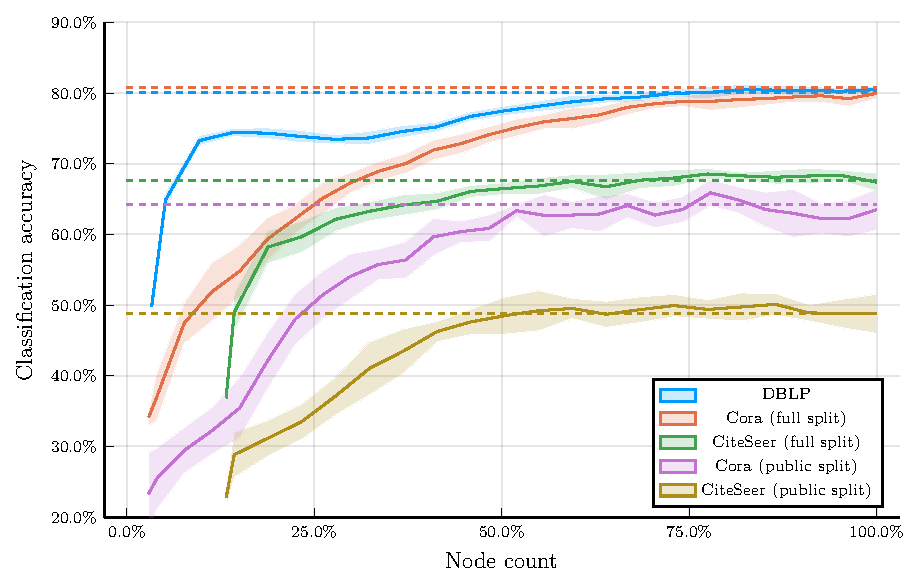
\includegraphics[width=\linewidth]{images/adaptive-coarsening/adaptive-coarsening.pdf}
  \caption{Adaptive coarsening results}
  \label{fig:adaptive-coarsening}
\end{figure}

\subsection{Relation to graph properties}

\todo[inline]{Compare the adaptive coarsening with local graph measures of graph homophilly}

\subsection{Comparison of coarsening approaches}
\todo[inline]{Compare the coarsenings measured by the graphs from previous section}
